\section{Gyrosensor Programmierung (Koch)}
Zu Beginn des Projekts war geplant den Gyrosensor MPU6050 zu nutzen, um die Position der Geschützplattform zu bestimmen, da eine kontinuierliche Bewegung um die eigene Achse aufgrund der Kabel nicht möglich ist. Dabei sollte der Sensor über den I2C-Bus mit dem Raspberry Pi 5 verbunden werden, um die Daten auszulesen und zu verarbeiten.
Der MPU6050 ist dabei ein 3-Achsen-Gyroskop und 3-Achsen-Beschleunigungssensor, welcher entsprechende Drehbewegungen und Beschleunigungen entlang der Raumachsen messen kann, welche für eine genaue Winkelbestimmung notwendig sind.

Nach kurzem Einlesen in die Dokumentation waren erste Rohdaten leicht auszulesen. Diese Rohdaten liegen in Form von 16 Bit in zwei Registern bereit und haben die Einheit $\mathit{LSB/g}$ für die Beschleunigungswerte und $\mathit{LSB/^\circ s}$ für die Gyroskop-Werte. Dies gilt es in tatsächliche physikalische Größen umzuwandeln, was bei unserem Projekt letztlich einem Winkel entspricht. 
Um die Beschleunigungswerte nutzen zu können, muss dafür mittels des Skalierungsfaktors die Fallbeschleunigung $\mathit{g}$ errechnet werden, indem man den erhaltenen Wert $x/16384$ rechnet. Die $16384$ ergeben sich aus der Dokumentation und entsprechen den LSB bei einem Messbereich von $\pm2g$, welches der Standardauflösung entspricht und auch die höchste Auflösung des MPU6050 für ist.
Ähnlich wird nun auch Winkelgeschwindigkeit ($\mathit{^\circ s}$) errechnet. Hierbei beträgt der Teiler standardmäßig $131$. \cite[S. 12-13]{raspberry_invensense_mpu6050_datasheet} 

Nach der Umrechnung der Rohdaten in physikalische Größen können nun die Neigungswinkel (Roll- und Pitch-Winkel) des Sensors berechnet werden. Diese ergeben sich aus der Richtung der Erdbeschleunigung relativ zum Sensor. 

Dazu wird die Erweiterung des Arkustangens genutzt, genauer gesagt die Funktion \texttt{atan2}, da sie im Gegensatz zum gewöhnlichen Arctangens auch die Orientierung in allen vier Quadranten berücksichtigt und somit stabile Winkelwerte über den gesamten Bereich von $-180^\circ$ bis $+180^\circ$ liefert. \cite{raspberry_matlab_atan2}

Die Winkelberechnung erfolgt nach der Formel \ref{eq:norms_to_angle}:

\begin{gather}
    \begin{aligned}
    \varphi_\text{pitch} &= \arctan2\left(a_x,\sqrt{a_y^2 + a_z^2}\right) \cdot \frac{180^\circ}{\pi} \\
    \varphi_\text{roll}  &= \arctan2\left(a_y, a_z\right) \cdot \frac{180^\circ}{\pi}
    \end{aligned}
    \label{eq:norms_to_angle}
\end{gather}


Hierbei sind $a_x$, $a_y$ und $a_z$ die normierten Beschleunigungswerte in $\mathit{g}$-Einheiten (berechnet aus den Rohwerten durch Division durch $16384$). 

Die $atan2$-Funktion liefert den Winkel zwischen der positiven $x$-Achse und dem Punkt $(x, y)$ in der Ebene, wodurch Sprünge oder Mehrdeutigkeiten bei $90^\circ$ vermieden werden. \cite{raspberry_matlab_atan2}

Nachdem der Term im Code implementiert wurde, konnte ein starkes Rauschen beobachtet werden, was zunächst auf natürliche Schwankungen des Sensors zurückgeführt wurde, weshalb sich dazu entschieden wurde zuerst einen Komplementärfilter zu implementieren,
welcher allerdings das Problem nur bedingt beheben konnte. Deshalb wurde auch noch der Kalman-Filter ausgetestet, wodurch auch eine starke  Rauschunterdrückung festgestellt werden konnte, doch auch hier zeichnete sich ein überdurchschnittliches Rauschverhalten ab, weshalb der Fehler nicht mehr auf ein natürliches Rauschen zurückzuführen war.
Daraufhin wurde auch ein zweiter MPU6050 getestet, welcher ebenfalls dieses Verhalten aufwies, wodurch klar wurde, dass es sich hierbei um einen Programmierfehler handeln muss. Dieser konnte nach einiger Zeit auch herausgefunden werden und lag an der Interpretation der Rohdaten, 
welche fälschlicherweise als \texttt{int16\_t} statt \texttt{uint16\_t} interpretiert wurden.

Aufgrund der aufgewendeten Zeit für die Implementierung des Kalman-Filters sollte dieser aber trotzdem Anwendung im Projekt finden und wird in \ref{sec:kalman_filter} behandelt.

Wie Eingangs erwähnt, sollte der Gyrosensor MPU6050 genutzt werden, um die Position der Geschützplattform zu bestimmen, wofür der Winkel der Drehung um die eigene Achse benötigt wird. Dabei stellte sich heraus das der MPU6050 für diesen Wert zu einem starken Drift neigt, weshalb empfohlen wird diesen mit einem Magnetometer zu kombinieren \cite[S. 26]{raspberry_invensense_mpu6050_datasheet}.
Zur gleichen Zeit stellte sich heraus, dass diese Funktionalität nicht benötigt wird, da über die Servo-Motoren bereits ein Nullpunkt definiert werden konnte, weshalb der Gyrosensor letztlich nur noch für die Neigung der Geschützplattform genutzt wird, um diese als Debug-Information auf dem Webserver \ref{sec:Webserver} anzuzeigen.

\begin{samepage}
    \subsection{Kalman Filter Implementierung (Koch)}
    \label{sec:kalman_filter}
    Der Kalman-Filter ist ein Algorithmus zur Schätzung des Zustands eines dynamischen Systems. Er nutzt Messwerte mit einem mathematischen Modell, um aus verrauschten Daten optimale Schätzungen zu erzeugen und zu filtern, was insbesondere bei Sensoren mit Rauschen, wie dem MPU6050, von Bedeutung ist \cite{raspberry_rwth_kalman_2025}.
    In der Abbildung \ref{fig:pitch_roll_vergleich} ist sowohl für den Roll, als auch den Pitch ein signifikanter Unterschied zwischen den Rohdaten und den gefilterten Daten zu erkennen. Die ersten Schwankungen der gefilterten Werte sind vermutlich darauf zurückzuführen, dass der Kalmanfilter mit wenig Referenzwerten nur ungenaue Schätzungen liefern kann, weshalb die Schätzungen auch erst mit steigender Anzahl an Werten genauer werden.
    Der Pitch konnte mithilfe des Kalmanfilters eine Rauschreduktion von $59.4\%$ erzielen und für den Roll $37.4\%$ bei jeweils $100$ Testwerten.

    Aufgrund der Art wie der Gyrosensor auf dem Geschützarm montiert ist, ist für die Neigung allerdings nur der Roll-Wert von Bedeutung.


    \begin{figure}[H]
        \centering
        % Bild für Pitch
        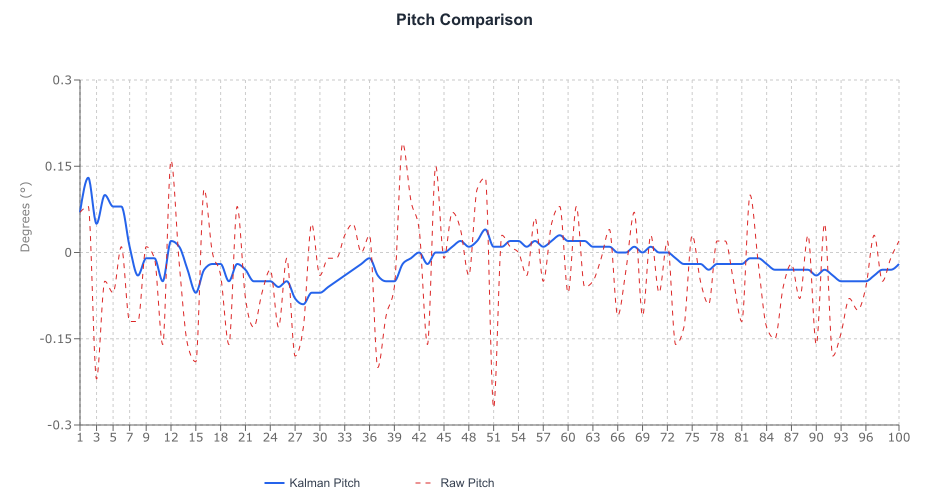
\includegraphics[width=0.8\textwidth]{images/kalman_comparison_pitch_2025-06-23.png}
        \vspace{1em} 
        
        % Bild für Roll
        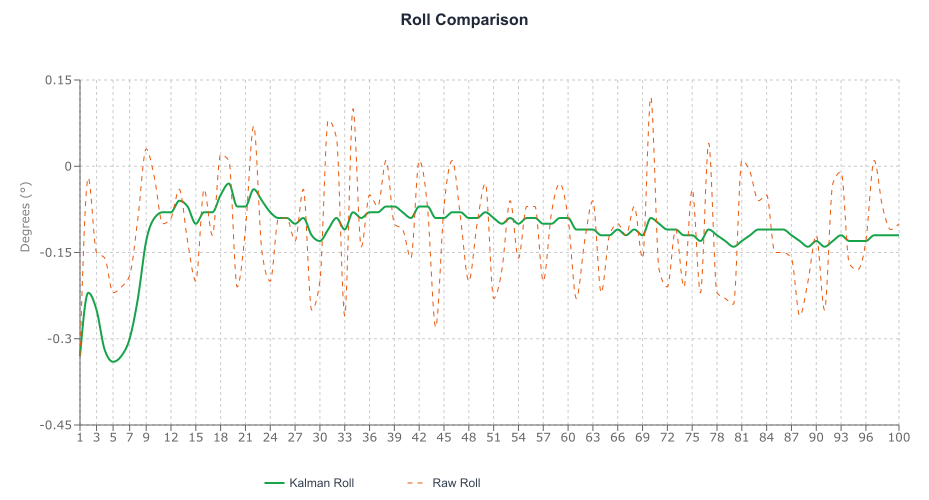
\includegraphics[width=0.8\textwidth]{images/kalman_comparison_roll_2025-06-23.png}
        
        \caption{Vergleich der Rohdaten und Kalman-Filter geschätzten Werte für Pitch und Roll}
        \label{fig:pitch_roll_vergleich}
    \end{figure}

\end{samepage}

